\documentclass[ngerman={babel}, utf8, bigger, xcolor={table,dvipsnames}, ompress, hyperref={bookmarks,colorlinks}]{beamer}

\usepackage{tikz}
\usetikzlibrary{positioning}

\title[Embedded Systems]{Software Engineering in Embedded Systems}
\author{Stephan Heidinger}
\date{Datum} %hier Datum des Vortrags einfügen
\institute[Seng-Seminar]{Seminar: Software Engineering \\ Fachbereich für Informatik und Informationssysteme \\ Universtität Konstanz}
%\setbeameroption{}
%\setbeamerfont{}{}
%\setbeamercolor{}{}
%\setbeamertemplate{}{}

%\usetheme{AnnArbor} %mit farbanpassung evtl
%\usetheme{Antibes}
%\usetheme{Berkeley} %mit sidebar, aber wenig struktur
%\usetheme{Hannover} %wie berkeley, aber weniger zeug
%\usetheme{Marburg} %pornosidebar
%\usetheme{Berlin} %"history" im header
%\usetheme{Boadilla} %nur footer, der aber gut
%\usetheme{CambridgeUS} %←←←←←schick
%\usetheme{Madrid}

%\usetheme{Goettingen}

%\usecolortheme{}
%\useinnertheme{}
%\useoutertheme{}
%\usefontheme{}

%setze normale navileiste auf null
%\setbeamertemplate{footline}{} \setbeamertemplate{navigation symbols}{}
%füge neue Navigationsleiste in die sidebar ein, die nur overlay und frame hat
%\setbeamertemplate{sidebar left}{\vspace*{\fill} \scalebox{1}[2]{\insertslidenavigationsymbol} \scalebox{1}[2]{\insertframenavigationsymbol}}

%standardoverlayreihenfolge: aktuelles overlay und auf allen danach
\beamerdefaultoverlayspecification{<+->}
%dasselbe + highlight auf dem aktuellen
%\beamerdefaultoverlayspecification{<+-| alert@+>}
%unsichtbarer text ist halb sichtbar
\setbeamercovered{transparent=25}
%show note-slides
\setbeameroption{show notes}

%\usetheme{Antibes}
\usecolortheme{dove}
%\useinnertheme{circles}
\useoutertheme{sidebar}


\begin{document}

%colors for definition boxes
\setbeamercolor{defHeader}{fg=black,bg=red!80}
\setbeamercolor{defBody}{fg=blue,bg=red!40}
%colors for tables
\rowcolors{1}{black!20}{black!40}

%\AtBeginSection{% This will post whatever is inside at the beginning of each section, maybe use sidebar instead
%	\begin{frame}<beamer>{Gliederung}%nur für beamer, nicht für handout
%	\tableofcontents[currentsection]
%	\end{frame}
%}

\begin{frame}{}{}% Beginn der Titelfolie
\maketitle
\end{frame}% Ende der Titelfolie



\section{Motivation}
\begin{frame}{Embedded Systems - What's that? - I}
	\begin{beamerboxesrounded}[upper=defHeader, lower=defBody,shadow=true]{Definition}
	\emph{``An \textbf{embedded software} system is part of a hardware/software system that reacts to events in its environment. The software is `embedded' in the hardware. Embedded systems are nominaly real-time systems.''\\
		{\tiny Software Engineering, p.561, Edited by Ian Sommerville, Ninth Edition}}
	\end{beamerboxesrounded}
\end{frame}

\begin{frame}{Embedded Systems - What's that? - II}
	Embedded Systems \dots
	\begin{itemize}
		\item \dots respond to physical world
		\item \dots respond in real time (``have a \emph{deadline}'')%time in which the result is produced
		\item \dots often have little resources %(i.e. not `computers')
		\item \dots run on special purpose hardware
		\item \dots run in real-time operating system
	\end{itemize}
\end{frame}

\begin{frame}{Embedded Systems - What's that? - III}
	Examples for Embedded Systems:
	\begin{itemize}
		\item airbag
		\item cell phone / `modern' phone
		\item burglar alarm
		\item (fully automatic) coffee machine
		\item danger detection %(NPP, earthquake, \dots)
		\item \dots
	\end{itemize}
\end{frame}

\begin{frame}{Motivation}
	\onslide<+->{We see:}
	\begin{itemize}%[<+->]
		\item Embedded Systems are everywhere!
		\item There are probably more Embedded Systems than computers out there!
	\end{itemize}
	\onslide<+->{We realize:}
	\begin{itemize}%[<+->]
		\item Man, they must be important.
		\item There sure is some money in this. %c-programming, special skills
	\end{itemize}
\end{frame}

%\section*{Outline}
\begin{frame}<beamer>{Outline}
\tableofcontents
\end{frame}

\section{Embedded Systems}
\begin{frame}{Problems}
	\begin{itemize}
		\item deadlines
		\note<.>{\textbf{deadlines:}\\ hard systems: deadline not met, failure\\ soft system: deadline not met, bad results}
		\item environment
		\note<.>{\textbf{environment:}\\ is unpredictable \\ embS $\Rightarrow$ concurrent}
		\item continuosity
		\note<.>{\textbf{continuosity:}\\ embS $\Rightarrow$ does not normaly terminate \\ software has to be reliable \\ update while operating}
		\item direct hardware interaction
		\note<.>{\textbf{direct hardware interaction:}\\ uncommon hardware (i.e. detonator in airbag) \\ speed issues (hardware is faster)}
		\item safety \& reliability
		\note<.>{\textbf{safety \& reliability:}\\ cost of failure high \\ either economical or in human life}
	\end{itemize}
\end{frame}

\section{Embedded Systems design}
\begin{frame}{Things to consider}
	\begin{itemize}
		\item design and performance of system hardware
		\note<.>{\textbf{design and performance of system hardware:}\\What hardware to use? \\ What is to be implemented in software, what in hardware}
		\item power consumption
		\note<.>{\textbf{power consumption:}\\ especially in mobile products (cells phones etc)}
		\item special purpose hardware
		\note<.>{\textbf{special purpose hardware:}\\ do we need special hardware? \\ design special hardware? \\ replace software by hardware?}
		\item stimuli:
		\note<.>{\textbf{stimuli:}\\ describe behaviour of system by listing received stimuli and reactions \\ stimuli = signals \\}
			\begin{enumerate}
				\item periodic stimuli
				\note<.>{\textbf{periodic stimuli:}\\occur at predictable intervalls \\ predefined reaction per stimulus \\ i.e. polling}
				\item aperiodic stimuli
				\note<.>{\textbf{aperiodic stimuli:}\\ occurr irreagularly and unpredictably \\ often interrupts \\ i.e. alarms, failures, IO operation finished, etc}
				\note<.>{\textbf{stimuli list:}\\best practice: stimuli list with \textbf{all} stimuli. \\ example next slide}
			\end{enumerate}
	\end{itemize}
\end{frame}

\begin{frame}{Example: radiation warning system}
	%\usetikzlibrary{positioning}
\begin{tikzpicture}
%shielding
\only<2->\draw (-.1,-.1) rectangle (6.1,6.1);
%reactor
\only<2->\draw[fill] (3,3) circle (1);
\only<2->\node[draw,circle,fill] (reactor-icon) at (6.5,5.8) {};
\only<2->\node (reactor) [right=0cm of reactor-icon] {reactor};

%room 1
\only<3->\draw (0,3) rectangle (3,6);
\only<3->\node (room1) at (1.5,4.5) {room 1};
\only<4->\draw[fill=blue!75] (2.5,5) circle (.1);
\only<4->\draw[fill=blue!75] (1,3.5) circle (.1);
%room 2
\only<3->\draw (0,0) rectangle (3,3);
\only<3->\node (room1) at (4.5,4.5) {room 2};
\only<4->\draw[fill=blue!75] (3.5,5) circle (.1);
\only<4->\draw[fill=blue!75] (5,3.5) circle (.1);
%room 3
\only<3->\draw (3,3) rectangle (6,6);
\only<3->\node (room1) at (1.5,1.5) {room 3};
\only<4->\draw[fill=blue!75] (2.5,1) circle (.1);
\only<4->\draw[fill=blue!75] (1,2.5) circle (.1);
%room 4
\only<4->\draw[fill=blue!75] (3.5,1) circle (.1);
\only<4->\draw[fill=blue!75] (5,2.5) circle (.1);
\only<3->\draw (3,0) rectangle (6,3);
\only<3->\node (room1) at (4.5,1.5) {room 4};

%legend
\only<4->\node[draw,circle,fill=blue!75] (sensor-icon) at (6.5,5.3) {};
\only<4->\node (reactor) [right=0cm of sensor-icon] {sensor};

%legend-border
\only<2->\draw (6.2,5) rectangle (8.2,6.1);
\end{tikzpicture}
\end{frame}

\begin{frame}{Example: Stimuli-List of a radiation warning system}
%	\rowcolors{1}{black!20}{black!40}
	\begin{tabular}{p{9em}p{13em}}
		\rowcolor{blue}\hline \textcolor{white}{Stimulus} & \textcolor{white}{Response} \\
		\pause single sensor positive & \pause flash warning light around sensor \\
		\pause both sensors in one area positive & \pause flash danger light, sound accoustic alarm \\
		\pause Voltage drop of 10-20\% & \pause switch to backup power; run power supply test \\
		\pause Voltage drop of more than 20\% & \pause switch to backup; run power supply test; call maintainer \\
%		\pause Panic button positive & \pause Initiate alarm; turn on lights around button; call police \\
	\end{tabular} \pause
\end{frame}

\section{Architectural design}

\section{Timing analysis}

\section{Real-time operating systems}


\begin{frame}{Last Slide}
	\vspace*{4em}{\huge Last Slide}
\end{frame}

%\subsection{noch mehr Text}
%\begin{frame}{Titel}{Untertitel} %allgemeine Folie
%	mehr text
%\end{frame}

\end{document}
